\documentclass{report}
\usepackage{amsmath,amsthm,amssymb}
\usepackage{mathtext}
\usepackage{graphicx}
\graphicspath{{bur_img/}}
\DeclareGraphicsExtensions{.jpg}
\usepackage[T1]{fontenc}
\usepackage{lmodern}
\usepackage[utf8]{inputenc}
\usepackage[english,russian]{babel}
\usepackage[usenames,dvipsnames]{color}
\usepackage{alltt}
\usepackage{microtype}

\makeatletter
\renewcommand\@biblabel[1]{#1.\hfil}
\makeatother

\begin{document}
	
	\begin{titlepage}
		
		\begin{center}
			Министерство науки и высшего образования Российской Федерации
		\end{center}
		
		\begin{center}
			Федеральное государственное автономное образовательное учреждение высшего образования \\
			Национальный исследовательский Нижегородский государственный университет им. Н.И. Лобачевского
		\end{center}
		
		\begin{center}
			Институт информационных технологий, математики и механики
		\end{center}
		
		\vspace{4em}
		
		\begin{center}
			\textbf{\Large Отчет по лабораторной работе} \\
		\end{center}
		\begin{center}
			\textbf{\Large«Вычисление многомерных интегралов с использованием многошаговой схемы (метод трапеций).»} \\
		\end{center}
		
		\vspace{4em}
		
		\newbox{\lbox}
		\savebox{\lbox}{\hbox{text}}
		\newlength{\maxl}
		\setlength{\maxl}{\wd\lbox}
		\hfill\parbox{7cm}{
			\hspace*{5cm}\hspace*{-5cm}\textbf{Выполнила:} 
			\newline студентка группы 381808-1 
			\newline Бурмистрова Е. О.
			\newline
			\newline
			\hspace*{5cm}\hspace*{-5cm}\textbf{Проверил:}
			\newline доцент кафедры МОСТ, 
			\newline кандидат технических наук 
			\newline Сысоев А. В.
		}
		\vspace{\fill}
		
		\begin{center} Нижний Новгород \\ 2021 \end{center}
		
	\end{titlepage}
		\setcounter{page}{2}
	
	% Содержание
	\tableofcontents
	\newpage

% Введение
\section*{Введение}
\addcontentsline{toc}{section}{Введение}
\par В настоящее время использование численных методов для решения некоторых математических задач даёт возможность ускорить вычисления в ситуациях, когда точность получаемых результатов не критична.
    
\par В данной работе рассматривается параллельное вычисление многомерных (1,2 и 3 порядков) интегралов методом трапеций, который крайне редко применяется в работе с интегралами 3 и более высоких порядков и не так часто используется при решении интегралов 2 порядка.
 
\par В рамках решения задачи были рассмотрены и применены такие технологии, как OpenMP, Thread Building Blocks (TBB), а также std::thread.
\newpage
% Постановка задачи
\section*{Постановка задачи}
\addcontentsline{toc}{section}{Постановка задачи}
В данной лабораторной работе было необходимо реализовать вычисление интегралов 1-3 порядков методом трапеций:
\begin{itemize}
\item последовательно;
\item с использованием библиотеки OpenMP;
\item с использованием библиотеки Thread Building Blocks (TBB);
\item с использованием встроенных возможностей параллельной разработки языка с++ - std::thread
\end{itemize}
\newpage
% Метод решения
\section*{Метод решения}
\addcontentsline{toc}{section}{Метод решения}
\par Прежде чем переходить к рассмотрению конкретного метода не будет лишним вспомнить, что представляет собой определённый интеграл на некотором конечном отрезке с геометрической точки зрения. Численное значение такого интеграла попросту равно площади под его графиком на указанном отрезке. 

\par В самом простом случае данную площадь можно представить (для значительного упрощения вычислений) в виде некоторого разбиения её на прямоугольники, количество которых прямо пропорционально точности результирующей площади.
Аналогично работает метод трапеций. Единственное его отличие от метода прямоугольников состоит в том, что за счёт скошенной верхушки каждый фрагмент будет плотнее прилегать к исходной кривой; следовательно, просуммировав все части разбиения, получим более точный результат.

\textbf{Side note : }  Если принимать во внимание особенности рассмотренных выше методов, можно понять, почему метод трапеций почти не используется для вычисления интегралов 2 и более старших порядков. => использование мной смеси нескольких способов с методом трапеций в осонове.
Метод трапеций представляет собой:
\begin{itemize}
\item в одномерном случае:
\begin{center}
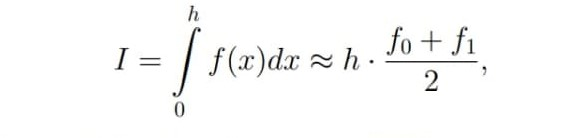
\includegraphics[scale=0.8]{bur_img/onedim.jpg}
\end{center}
\item в многомерном случае:
\begin{center}
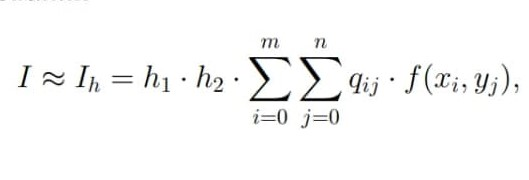
\includegraphics[scale=0.8]{bur_img/multidim.jpg}
\end{center}
\begin{center}
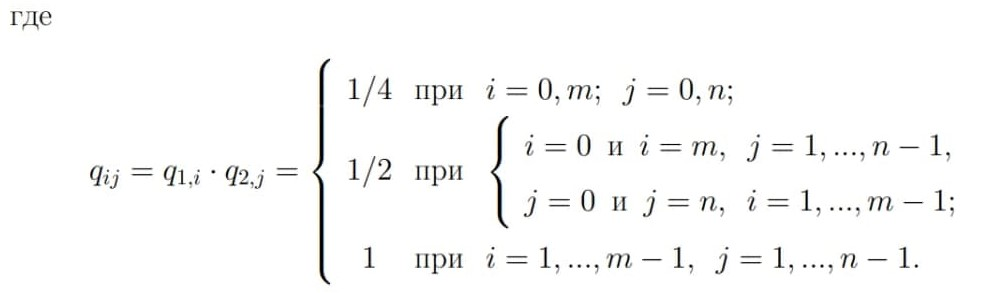
\includegraphics[scale=0.6]{bur_img/system.jpg}
\end{center}
\end{itemize}
\newpage

% Схема распараллеливания
\section*{Схема распараллеливания}
\addcontentsline{toc}{section}{Схема распараллеливания}
\par На начальном этапе имеем некоторый набор функций от 1-й, 2-х и 3-х переменных.

\par В каждой реализации пользуемся основными формулами и методами: формула трапеций, квадратурные формулы, метод ячеек.
Получаем одномерные, двумерные и трёхмерные циклы для соответствующих интегралов.
\begin{enumerate} 
\item OpenMP: пользуемся \begin{alltt}parallel_for\end{alltt} с редукцией по сумме.
\item TBB: пользуемся \begin{alltt}tbb::parallel_reduce\end{alltt} по сумме.
\item std::thread ... .
\end{enumerate}
\newpage

% Описание программной реализации
\section*{Описание программной реализации}
\addcontentsline{toc}{section}{Описание программной реализации}
В данной работе реализованы 2 основных метода :
\begin{alltt}
double SolveParallel(const std::vector<std::pair<int, int>>& bord,
    std::function<double(double, double, double)> f){}; - для вычисления интегралов \\ с опрецией "умножение"
double SolveParallelSum(const std::vector<std::pair<int, int>>& bord,
    std::function<double(double, double, double)> f){}; - для вычисления интегралов \\ с опрецией "сложение"
\end{alltt}
В последовательной реализации так же используется метод:
\begin{alltt}
double CheckCoeff(int i, const std::pair<int, int>& pair){}; - для  формирования \\ коэффициента q формулы метода трапеций.
\end{alltt}
\newpage
% Подтверждение корректности
\section*{Подтверждение корректности}
\addcontentsline{toc}{section}{Подтверждение корректности}
Для подтверждения корректности работы были созданы 5 тестов.
\begin{enumerate}
\item Sequential и OpenMP: 
        \begin{alltt}
        TEST(Parallel_Operations_OpenMP, Test_OneDim) {}
        TEST(Parallel_Operations_OpenMP, Test_TwoDim) {}
        TEST(Parallel_Operations_OpenMP, Test_ThreeDim) {}
        TEST(Parallel_Operations_OpenMP, Test_TwoDimSum) {}
        TEST(Parallel_Operations_OpenMP, Test_ThreeDimSum) {}
        \end{alltt}
\item TBB:
        \begin{alltt}
        TEST(Parallel_Operations_TBB, Test_OneDim) {}
        TEST(Parallel_Operations_TBB, Test_TwoDim) {}
        TEST(Parallel_Operations_TBB, Test_ThreeDim) {}
        TEST(Parallel_Operations_TBB, Test_TwoDimSum) {}
        TEST(Parallel_Operations_TBB, Test_ThreeDimSum) {}
        \end{alltt}        
        Именно с их помощью процесс отладки становится нативным и менее затратным по времени.
\end{enumerate}
\newpage
% Результаты экспериментов
\section*{Результаты экспериментов}
\addcontentsline{toc}{section}{Результаты экспериментов}
Эксперименты проводились на ПК с следующей конфигурацией:
\begin{itemize}
\item Операционная система: Windows 10
\item Процессор: Intel(R) Core™ i3 M 380 CPU @ 2.53 GHz
\item ОЗУ 6 гб
\item Версия Visual Studio: 2017
\item Количество разбиений : 999
\end{itemize}
\begin{figure}[ht]
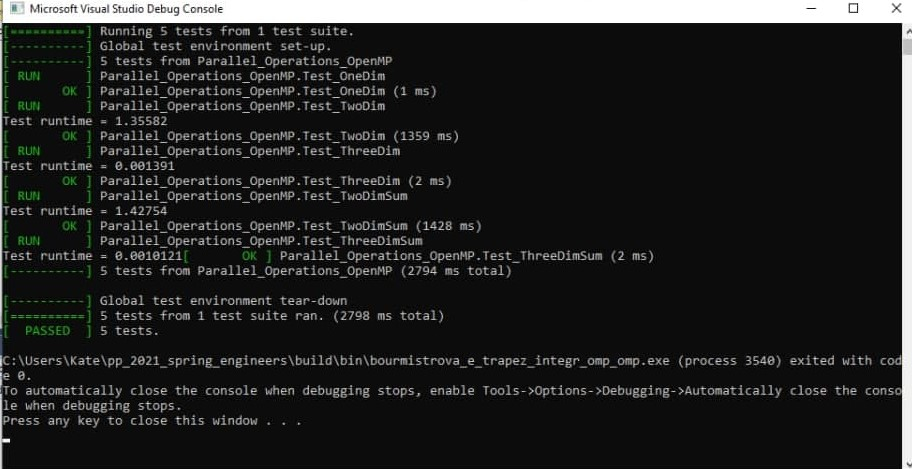
\includegraphics[scale=0.6]
{bur_img/ph1.jpg}
\caption{1 thread OMP}
\end{figure}
\begin{figure}[ht]
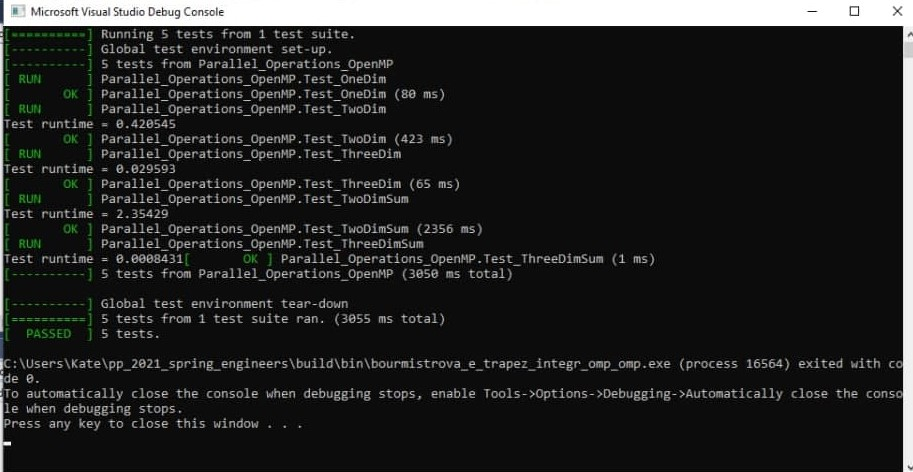
\includegraphics[scale=0.6]
{bur_img/ph6.jpg}
\caption{6 threads OMP}
\end{figure}
\begin{figure}[ht]
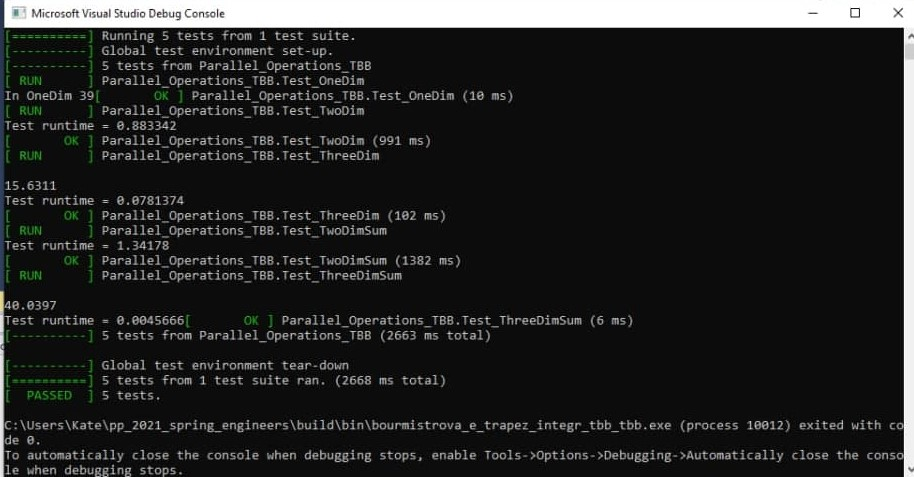
\includegraphics[scale=0.6]
{bur_img/phtbb.jpg}
\caption{auto chosen threads TBB}
\end{figure}
\newpage
% Заключение
\section*{Заключение}
\addcontentsline{toc}{section}{Заключение}
Реализованные алгоритмы вычисления многомерных интегралов позволяют оценить разность в производительности
для данных подходов, изучить конкретные примеры их реализаций.
\newpage
% Список литературы
\begin{thebibliography}{1}
\addcontentsline{toc}{section}{Список литературы}
\bibitem{math1}
Блюмин А.Г., Федотов А.А., Храпов П.В.
\textit{Численные методы вычисления интегралов и решения задач для обыкновенных дифференциальных уравнений Методические указания
к выполнению лабораторных работ по курсу «Численные методы»}
\bibitem{tbb1}
А.В. Сысоев, И.Б. Мееров, А.А. Сиднев
\textit{Средства разработки параллельных программ для систем
с общей памятью. Библиотека Intel Threading Building 
Blocks}
\bibitem{shared1}
К.В. Корняков, В.Д. Кустикова, И.Б. Мееров, А.А. Сиднев, А.В. Сысоев, А.В. Шишков
\textit{ИНСТРУМЕНТЫ ПАРАЛЛЕЛЬНОГО ПРОГРАММИРОВАНИЯ В СИСТЕМАХ С ОБЩЕЙ ПАМЯТЬЮ}
\bibitem{math2}
Квадратурные (кубатурные) методы численного интегрирования по отрезку (многомерному кубу)
\\\texttt{https://clck.ru/VJgXW}
\end{thebibliography}
\newpage
% Приложение
\section*{Приложение}
\addcontentsline{toc}{section}{Приложение}
 	\subsection*{trapezoid\_integral.zpp}
 	\begin{verbatim}
// Copyright 2021 Ekaterina Burmistrova

#include <omp.h>
#include <vector>
#include <string>
#include <random>
#include <iostream>
#include <functional>
#include "./../../modules/task_1/bourmistrova_e_tr_int/trapezoid_integral.h"

double CheckCoeff(int i, const std::pair<int, int>& pair) {
    double qju = 1.00;
    if (i == pair.first || i == pair.second)
        qju *= 0.5;
    return qju;
}

double SolveSequential(const std::vector<std::pair<int, int>>& bord,
    std::function<double(double, double, double)> f) {   // add n,m,k;
    double sum = 0;
    int i = 0, j = 0, k = 0;
    if (bord.size() == 1) {  // ONE DIMENSION
        // double h = (bord[0].second - bord[0].first) / n;
        for (i = bord[0].first; i < bord[0].second; i++) {
            sum += ((f(i, 1, 1) + f(i + 1, 1, 1)) / 2);
        }
    } else if (bord.size() == 2) {  // TWO DIMENSIONS
        double q0 = 1, q1 = 1;
        // double h1 = (bord[0].second - bord[0].first) / n;
        // double h2 = (bord[1].second - bord[1].first) / k;
        for (i = bord[0].first; i < bord[0].second+1; i++) {
            q0 = CheckCoeff(i, bord[0]);
            for (j = bord[1].first; j < bord[1].second+1; j++) {
                    q1 = CheckCoeff(j, bord[1]);
                    sum += q0 * q1 * f(i, j, 1);
            }
        }
    } else {  // THREE DIMENSIONS
        double q0 = 1, q1 = 1, q2 = 1;
        // int h1 = (bord[0].second - bord[0].first) / n;
        // int h2 = (bord[1].second - bord[1].first) / m;
        // int h3 = (bord[2].second - bord[2].first) / k;
        for (i = bord[0].first; i < bord[0].second + 1; i++) {
            q0 = CheckCoeff(i, bord[0]);
            for (j = bord[1].first; j < bord[1].second + 1; j++) {
                q1 = CheckCoeff(j, bord[1]);
                for (k = bord[2].first; k < bord[2].second + 1; k++) {
                        q2 = CheckCoeff(k, bord[2]);
                        sum += q0 * q1 * q2 * f(i, j, k);
                }
            }
        }
    }
    return sum;
}
 	\end{verbatim}
  	\subsection*{trapez\_integr.cpp}
 	\begin{verbatim}
// Copyright 2021 Ekaterina Burmistrova
#include <omp.h>
#include <vector>
#include <string>
#include <random>
#include <iostream>
#include <functional>
#include "./../../modules/task_2/bourmistrova_e_trapez_integr_omp/trapezoid_integral_omp.h"


double CheckCoeff(double i, int s_pr) {
    double qju = 1.00;
    if (i = 0 || i == s_pr)
        qju *= 0.5;
    return qju;
}

double OneDimIntegr(const std::vector<std::pair<int, int>>& bord,
    std::function<double(double, double, double)> f,
    int set_prec, int pr1, double pr2, double s, int b) {
    double tr_sum = 0;
    omp_set_num_threads(6);
    #pragma omp parallel for private(pr1, pr2) reduction(+:tr_sum)
    for (pr1 = 0; pr1 < set_prec; pr1++) {
        pr2 = bord[b].first + pr1 * s;
        tr_sum += ((f(pr2, 1, 1) + f(pr2 + s, 1, 1)) / 2) * s;
    }
    return tr_sum;
}
double SolveParallel(const std::vector<std::pair<int, int>>& bord,
    std::function<double(double, double, double)> f) {
    omp_set_num_threads(6);
    double tr_sum = 0;
    double m = 1;
    int i = 0, j = 0, k = 0;
    double q0 = 0, q1 = 0, q2 = 0;
    double x = 0, x1 = 0, x2 = 0, x3 = 0, x4 = 0, x5 = 0;
    int set_precision = 1000;
    double s = (bord[0].second -
        bord[0].first)/ static_cast<double>(set_precision);
    if (bord.size() == 1) {  // ONE DIMENSION
        tr_sum = OneDimIntegr(bord, f, set_precision, i, x, s, 0);
    } else if (bord.size() == 2) {  // TWO DIMENSIONS
        double s2 = (bord[1].second -
            bord[1].first) / static_cast<double>(set_precision);
        #pragma omp parallel for reduction(+:tr_sum)
        for (i = 0; i < set_precision + 1; i++)
            for (j = 0; j < set_precision + 1; j++) {
                x = bord[0].first + i * s;
                x1 = x + i * s;
                x2 = bord[1].first + j * s2;
                x3 = x2 + j * s2;
                tr_sum += (f(x, x2, 1) + f(x, x3, 1) +
                    f(x1, x2, 1) + f(x1, x3, 1));
            }
        tr_sum = ((s * s2) / 4) * tr_sum;
    } else {  // THREE DIMENSIONS
        double s2 = (bord[1].second -
            bord[1].first) / static_cast<double>(set_precision);
        double s3 = (bord[2].second -
            bord[2].first) / static_cast<double>(set_precision);
        double q0 = 1, q1 = 1, q2 = 1;
        double tmp = 0;
        #pragma omp parallel for reduction(+:tr_sum)
        for (i = 0; i < set_precision; i++) {
            x = bord[2].first + i * s3;
            tr_sum += ((f(x, 1, 1) + f(x + s3, 1, 1)) / 2)*s3;
        }
        #pragma omp parallel for reduction(+:tmp)
        for (i = 0; i < set_precision; i++) {
            x = bord[1].first + i * s2;
            tmp += ((f(1, x, 1) + f(1, x+s2, 1)) / 2)*s2 * tr_sum;
        }
        #pragma omp parallel for reduction(+:tr_sum)
        for (i = 0; i < set_precision; i++) {
            x = bord[0].first + i * s;
            tr_sum += ((f(1, 1, x) + f(1, 1, x+s3)) / 2)*s*tmp;
        }
    }
    return tr_sum;
}
double SolveParallelSum(const std::vector<std::pair<int, int>>& bord,
    std::function<double(double, double, double)> f) {
    omp_set_num_threads(6);
    double tr_sum = 0;
    double m = 1;
    int i = 0, j = 0, k = 0;
    double q0 = 0, q1 = 0, q2 = 0;
    double x = 0, x1 = 0, x2 = 0, x3 = 0;
    int set_precision = 1000;
    double s = (bord[0].second -
        bord[0].first) / static_cast<double>(set_precision);
    if (bord.size() == 2) {  // TWO DIMENSIONS
    double s2 = (bord[1].second -
        bord[1].first) / static_cast<double>(set_precision);
    for (i = 0; i < set_precision + 1; i++)
        #pragma omp parallel for schedule(static) reduction(+:tr_sum)
        for (j = 0; j < set_precision + 1; j++) {
            x = bord[0].first + i * s;
            x1 = x + i * s;
            x2 = bord[1].first + j * s2;
            x3 = x2 + j * s2;
            if (i == 0 || i == set_precision)
                m *= 0.5;
            if (j == 0 || j == set_precision)
                m *= 0.5;
            tr_sum += m * (f(x, x2, 1) + f(x1, x3, 1) +
                f(x1, x2, 1) + f(x1, x3, 1));
            m = 1;
        }
    tr_sum = ((s * s2)/7.5) * tr_sum;
    } else {  // THREE DIMENSIONS
        double s2 = (bord[1].second -
            bord[1].first) / static_cast<double>(set_precision);
        double s3 = (bord[2].second -
            bord[2].first) / static_cast<double>(set_precision);
        double m = 1;
        double q0 = 1, q1 = 1, q2 = 1;
        double tmp = 0;
#pragma omp parallel for reduction(+:tr_sum)
        for (i = 0; i < set_precision; i++) {
            x = bord[2].first + i * s3;
            tr_sum += ((f(x, 1, 1) + f(x + s3, 1, 1)) / 2) * s3;
        }
#pragma omp parallel for reduction(+:tr_sum)
        for (i = 0; i < set_precision; i++) {
            x = bord[1].first + i * s2;
            tr_sum += ((f(1, x, 1) + f(1, x + s2, 1)) / 2) * s2;
        }
#pragma omp parallel for reduction(+:tr_sum)
        for (i = 0; i < set_precision; i++) {
            x = bord[0].first + i * s;
            tr_sum += ((f(1, 1, x) + f(1, 1, x + s3)) / 2) * s;
        }
    }
    return tr_sum;
}
\end{verbatim}
  	\subsection*{tr\_int\_tbb.cpp}
 	\begin{verbatim}
 	// Copyright 2021 Ekaterina Burmistrova
#include <tbb/tbb.h>
#include <vector>
#include <string>
#include <random>
#include <iostream>
#include <functional>
#include "./../../modules/task_3/bourmistrova_e_trapez_integr_tbb/tr_int_tbb.h"


double CheckCoeff(double i, int s_pr) {
    double qju = 1.00;
    if (i = 0 || i == s_pr)
        qju *= 0.5;
    return qju;
}
double OneDimIntegr(const std::vector<std::pair<int, int>>& bord,
    std::function<double(double, double, double)> f,
    int set_prec, int pr1, double pr2, double s, int b) {
    //// tbb::task_scheduler_init(6);  // automatic
    double tr_sum = tbb::parallel_reduce(tbb::blocked_range<int>(0, set_prec),
        0.0,
        [&](tbb::blocked_range<int> r, double running_total){
            for (pr1 = r.begin(); pr1 < r.end(); ++pr1) {
                pr2 = bord[b].first + pr1 * s;
                running_total += ((f(pr2, 1, 1) + f(pr2 + s, 1, 1)) / 2) * s;
            }
            return running_total;
        }, std::plus<double>());
    return tr_sum;
}
double SolveParallel(const std::vector<std::pair<int, int>>& bord,
    std::function<double(double, double, double)> f) {
    //// tbb::task_scheduler_init(6);  // automatic
    double tr_sum = 0;
    double m = 1;
    int i = 0, j = 0, k = 0;
    double q0 = 0, q1 = 0, q2 = 0;
    double x = 0, x1 = 0, x2 = 0, x3 = 0, x4 = 0, x5 = 0;
    int set_precision = 1000;
    double s = (bord[0].second -
        bord[0].first) / static_cast<double>(set_precision);
    if (bord.size() == 1) {  // ONE DIMENSION
        // std::cout << "In OneDim ";
        tr_sum = OneDimIntegr(bord, f, set_precision, i, x, s, 0);
        // std::cout << tr_sum;
    } else if (bord.size() == 2) {  // TWO DIMENSIONS
        double s2 = (bord[1].second -
            bord[1].first) / static_cast<double>(set_precision);
        tr_sum += tbb::parallel_reduce(tbb::blocked_range<int>(0,
            set_precision), 0.0,
            [&](tbb::blocked_range<int> rr, double running_total_o) {
                for (i = rr.begin(); i < rr.end()+1; ++i) {
                    running_total_o += tbb::parallel_reduce(
                        tbb::blocked_range<int>(0, set_precision), 0.0,
                        [&](tbb::blocked_range<int> r, double running_total) {
                            for (j = r.begin(); j < r.end()+1; ++j) {
                                x = bord[0].first + i * s;
                                // x1 = x + i * s;
                                x2 = bord[1].first + j * s2;
                                // x3 = x2 + j * s2;
                                if (i == 0 || i == set_precision)
                                    m *= 0.5;
                                if (j == 0 || j == set_precision)
                                    m *= 0.5;
                                running_total += m * f(x, x2, 1);
                                m = 1;
                            }
                            return running_total;
                        }, std::plus<double>());
                }
                return running_total_o;
            }, std::plus<double>());
        tr_sum = ((s * s2)/4) * tr_sum;
    } else {  // THREE DIMENSIONS
        double s2 = (bord[1].second -
            bord[1].first) / static_cast<double>(set_precision);
        double s3 = (bord[2].second -
            bord[2].first) / static_cast<double>(set_precision);
        double q0 = 1, q1 = 1, q2 = 1;
        double tmp = 0;
        tr_sum += tbb::parallel_reduce(tbb::blocked_range<int>(0,
            set_precision), 0.0,
            [&](tbb::blocked_range<int> r, double running_total) {
                for (i = r.begin(); i < r.end()+1; ++i) {
                    x = bord[2].first + i * s3;
                    running_total += ((f(x, 1, 1) + f(x + s3, 1, 1)) / 2) * s3;
                }
                return running_total;
            }, std::plus<double>());
        tmp += tbb::parallel_reduce(tbb::blocked_range<int>(0, set_precision),
            0.0,
            [&](tbb::blocked_range<int> r, double running_total) {
                for (i = r.begin(); i < r.end(); ++i) {
                    x = bord[1].first + i * s2;
                    running_total += ((f(1, x, 1) + f(1, x + s2, 1)) / 2) * s2;
                }
                return running_total;
            }, std::plus<double>());
        tr_sum *= tmp;
        tr_sum += tbb::parallel_reduce(tbb::blocked_range<int>(0,
            set_precision), 0.0,
            [&](tbb::blocked_range<int> r, double running_total) {
                for (i = r.begin(); i < r.end(); ++i) {
                    x = bord[0].first + i * s;
                    running_total += ((f(1, 1, x) + f(1, 1, x + s3)) / 2)*s;
                }
                return running_total;
            }, std::plus<double>());
        // std::cout << std::endl << tr_sum << std::endl;
        tr_sum = tr_sum / 2;
    }
    return tr_sum;
}
double SolveParallelSum(const std::vector<std::pair<int, int>>& bord,
    std::function<double(double, double, double)> f) {
    //// tbb::task_scheduler_init(6);  // automatic
    double tr_sum = 0;
    double m = 1;
    int i = 0, j = 0, k = 0;
    double q0 = 0, q1 = 0, q2 = 0;
    double x = 0, x1 = 0, x2 = 0, x3 = 0;
    int set_precision = 1000;
    double s = (bord[0].second -
        bord[0].first) / static_cast<double>(set_precision);
    if (bord.size() == 2) {  // TWO DIMENSIONS
        double s2 = (bord[1].second -
            bord[1].first) / static_cast<double>(set_precision);
        tr_sum += tbb::parallel_reduce(tbb::blocked_range<int>(0,
            set_precision), 0.0,
            [&](tbb::blocked_range<int> rr, double running_total_o) {
                for (i = rr.begin(); i < rr.end(); ++i)
                    running_total_o += tbb::parallel_reduce(
                        tbb::blocked_range<int>(0, set_precision), 0.0,
                        [&](tbb::blocked_range<int> r, double running_total) {
                            for (j = r.begin(); j < r.end(); ++j) {
                                x = bord[0].first + i * s;
                                x1 = x + i * s;
                                x2 = bord[1].first + j * s2;
                                x3 = x2 + j * s2;
                                if (i == 0 || i == set_precision)
                                    m *= 0.5;
                                if (j == 0 || j == set_precision)
                                    m *= 0.5;
                                running_total += m * (f(x, x2, 1) +
                                    f(x1, x3, 1) + f(x1, x2, 1) +
                                    f(x1, x3, 1));
                                m = 1;
                            }
                            return running_total;
                        }, std::plus<double>());
                return running_total_o;
            }, std::plus<double>());
        tr_sum = ((s * s2) / 10.5) * tr_sum;
    } else {  // THREE DIMENSIONS
        double s2 = (bord[1].second -
            bord[1].first) / static_cast<double>(set_precision);
        double s3 = (bord[2].second -
            bord[2].first) / static_cast<double>(set_precision);
        double m = 1;
        double q0 = 1, q1 = 1, q2 = 1;
        double tmp = 0;
        tr_sum += tbb::parallel_reduce(tbb::blocked_range<int>(0,
            set_precision), 0.0,
            [&](tbb::blocked_range<int> r, double running_total) {
                for (i = r.begin(); i < r.end(); ++i) {
                    x = bord[2].first + i * s3;
                    running_total += ((f(x, 1, 1) + f(x + s3, 1, 1)) / 2) * s3;
                }
                return running_total;
            }, std::plus<double>());
        tr_sum += tbb::parallel_reduce(tbb::blocked_range<int>(0,
            set_precision), 0.0,
            [&](tbb::blocked_range<int> r, double running_total) {
                for (i = r.begin(); i < r.end(); ++i) {
                    x = bord[1].first + i * s2;
                    running_total += ((f(1, x, 1) + f(1, x + s2, 1)) / 2) * s2;
                }
                return running_total;
            }, std::plus<double>());
        tr_sum += tbb::parallel_reduce(tbb::blocked_range<int>(0,
            set_precision), 0.0,
            [&](tbb::blocked_range<int> r, double running_total) {
                for (i = r.begin(); i < r.end(); ++i) {
                    x = bord[0].first + i * s;
                    running_total += ((f(1, 1, x) + f(1, 1, x + s3)) / 2) * s;
                }
                return running_total;
            }, std::plus<double>());
         // std::cout << std::endl <<  tr_sum << std::endl;
    }
    return tr_sum;
}
 	\end{verbatim}
	\end{document}